\chapter{Analyse}

\todo{Betrachtung wie Features gelernt werden können. Auf der Basis dann Gruppierung} Ein Gruppieren von Bildern anhand ihrer Deskriptoren ist ohne weitere Verarbeitung kaum möglich. Zum einen besitzen die Feature-Deskriptoren viele Komponenten, zum anderen liegen pro Bild selbst viele Deskriptoren vor (bei gängigen Größen ca. 20 - 3000 Deskriptoren).
Das Analysekapitel beginnt daher mit einem Überblick über das Themengebiet des maschinellen Lernens: Machine Learning. Hier handelt es sich um keine umfängliche Einführung. Es werden Methoden beleuchtet, die zur Komprimierung und Gruppierung von Daten, hier den Features, dienen und im weiteren der Arbeit verwendet werden. Anhand der Anforderungen und Annahmen wird dann ein unüberwachtes Lernverfahren vorgeschlagen, dass zu Gruppierung von Bildern dient und im folgenden ausgearbeitet und realisiert werden soll.
Das Kapitel Features beginnt mit einer Vorstellung einiger Feature-Detektoren bzw. Deskriptoren für unterschiedlicher Anwendungsfälle um in das Thema einzuführen. Heute ist es kaum vorstellbar, dass ein Feature-Deskriptor jeden möglichen Anwendungsfall abdecken kann. Im Folgenden soll daher der Fokus der Arbeit festgelegt werden: Sollen beispielsweise Gesichter oder Szenen erkannt werden? Sollen Objekte erkannt werden und wenn ja, beliebige Kategorien? Anhand der gewonnen Erkenntnisse wird dann entschieden, welche Eigenschaften der hier verwendete Feature-Deskriptor aufweisen soll bzw. muss. 

\section{Verwendung der GPU}

Zum Aufbauen eines Modells werden mehrere Zehn- bis Hunderttausend Features verarbeitet werden. Viele der Verfahren, die der Erzeugung solcher Modellen zu Grunde liegen, wurden in den vergangenen Jahren durch die Verwendung der GPU statt der CPU beschleunigt. Bei der Betrachtung geeigneter Ansätze wird daher auch berücksichtigt, ob und wie eine Beschleunigung durch parallele Verarbeitung erzielt werden kann. Gerade bei großen Datenmengen und einer enormen Datenparallelität können Probleme durch GPUs um ein vielfaches schneller gelöst werden als durch CPUs. Da Nvidias CUDA an der Hochschule Hannover sowohl gelehrt als auch zu Forschungszwecken genutzt wird und sich CUDA auch international in Forschung und Wirtschaft etabliert hat, soll die Plattform als technische Basis dienen. 

\section{Machine Learning}

Machine Learning ist ein Teilgebiet der künstlichen Intelligenz und wird genutzt um System zu entwerfen, die nicht explizit programmiert werden. Stattdessen Lernen diese Systeme: Lernen bedeutet in diesem Kontext, dass eine System durch eine Eingabe seine Struktur verändert, um so die erwartete Leistung zu steigern. Dabei ist Machine Learning ein interdisziplinäres Feld: Es sind sowohl Computerwissenschaften, Statistik als auch biologische und kognitive Wissenschaften involviert. Bisher haben sich viele Anwendungsfälle für Machine Learning Verfahren ergeben, die bis in den Alltag reichen. Einige Beispiele sind:

\begin{itemize}
	\item \textbf{Optical Character Recognition (OCR)} Unter OCR wird das Übersetzen eines (hand-)geschriebenen Textes in eine digitales Dokument bezeichnet. Beispielsweise kann so das Einfügen von Daten in CRM / ERP System automatisiert werden.
	\item \textbf{Spam Filterung} Das automatische Erkennen von unerwünschten E-Mails, die Werbung enthalten oder Betrugsversuche sind, ist inzwischen bei jedem Mail-Anbieter Teil des Angebots.
	\item \textbf{Spracherkennung} Auch eine Spracherkennung ist bereits auf den meisten digitalen Assistenten verfügbar und wird sogar zur Steuerung der häuslichen Elektronik verwendet.
	\item \textbf{Anomalie Erkennung} Digitale Geldtransaktionen werden heute von Algorithmen überwacht, die Abweichungen im Zahlungsverhalten beobachten. Wird eine ungewöhnlich hohe Summe überwiesen oder abgehoben, kann so informiert und auch interveniert werden.
\end{itemize}

All diese Verfahren Nutzen eine große Menge an Trainingsdaten, um so ein Modell zu generieren, welches eine Klassifizierung weiterer Daten ermöglicht. Beispielsweise müssen bei einem System zur Spam Filterung sowohl \glqq normale\grqq  als auch Spam E-Mails verwendet werden, eine Spracherkennung benötigt digitale Aufnahmen von Wörtern und Sätzen zum Lernen, etc.
Nach dem Aufbau des Modells findet dann durch das System die Klassifizierung von Test- bzw. realen Daten statt. Es wird beispielsweise bei OCR entschieden, welches digitale Pendant zum vorliegenden Zeichen gehört oder wie hoch die Wahrscheinlichkeit ist, dass es sich bei einer Mail um Spam handelt. Diese Trainings- und Testphase sind typisch für Machine Learning Verfahren. Allgemein eignet sich dieser Ansatz:

\begin{itemize}
	\item Um Beziehungen und Muster in den Daten zu entdecken, die nicht offensichtlich sind. Im Wesentlichen beschäftigt sich die Disziplin \textit{Data Mining} mit dieser Fragestellung und nutzt u.a. Machine Learning Verfahren.
	\item Wenn kein klassischer Algorithmus für die Problemstellung entworfen werden kann oder das Programm zu komplex ist, als das es von Menschen kodiert und gewartet werden könnte.
	\item Um neue Informationen einzubeziehen. Das Modell basiert auf den Daten, daher kann das System sich durch neue Daten verändern und so der Situation anpassen.
\end{itemize}

\subsection{Lernverfahren}

Je nach Fragestellung haben sich unterschiedliche Methodiken entwickelt, um den Lernprozess in einem System abzubilden. Im Wesentlichen werden drei Arten des maschinellen Lernens unterschieden:

\begin{itemize}
	\item \textbf{Überwachtes Lernen (supervised learning)} Ein überwachtes Lernverfahren soll eine Funktion $f$ lernen, die Eingaben ($x$) ihren Ausgaben ($y$) zuordnet, sodass gilt: $y = f(x)$ . Diese Funktion wird anhand von Trainingsdaten gelernt, die demzufolge aus Paaren von Eingaben und ihren dazugehörigen Ausgaben bestehen.
	\item \textbf{Unüberwachtes Lernen (unsupervised learning)} Ziel unüberwachter Lernalgorithmen ist es, großen Mengen von nicht kategorisierten Daten zu gruppieren oder zu komprimieren. Dadurch können Beziehungen in den Daten entdeckt bzw. kompaktere Darstellungen erreicht werden.
	\item \textbf{Verstärkendes Lernen (reinforcement learning)} Beim verstärkenden Lernen hat ein Agent die Aufgabe ein vorgegebenes Ziel zu erreichen, indem er mit seiner Umwelt agiert. Die Umwelt ist dabei eine Menge von Zuständen zwischen denen der Agent durch eine Aktion wechselt. Dabei hat jede Aktion eine Belohnungen oder Bestrafungen zufolge. Der Agent optimiert dann sein Verhalten, um die erhaltenen Belohnungen zu maximieren.
\end{itemize}

Beim überwachten Lernen ist es notwendig, dass sowohl Ursachen (Eingaben) als auch Effekte (Ausgaben) gemessen wurden. Beim unüberwachten Lernen hingegen sind die Eingaben latente Variablen. Das heißt sie sind nicht direkt gemessen worden, sondern durch mathematische Verfahren von Observationen abgeleitet. Dadurch ist ein exploratives Vorgehen möglich. Es können Beziehungen in den Daten entdeckt und Gruppierungen bzw. Klassifizierungen durchgeführt werden.

\subsection{Auswahl geeigneter Modelle}

\todo{Why unsupervised}
Bevor ein Modell ausgewählt wird, soll vorab ein Überblick über die verschiedenen Verfahren im Bereich des unüberwachten Lernens gegeben werden. Die Verfahren werden in die Kategorien \textit{Clustering} und \textit{Dimensionality Reduction (Reduzierung der Dimensionalität} eingeteilt. 

\textbf{Clustering-Verfahren} quantisieren die Daten in Gruppen. Eine Gruppe steht hier für ein semantisches Merkmal und vertritt eine Menge von konkreten Daten. Unter Clustering Verfahren fallen Algorithmen wie k-means, hierarchical clustering oder etwa das Gaussian Mixture Model. Ein Clustering Algorithmus hat in dem Kontext dieser Arbeit das Ziel, eine großen Menge Feature-Deskriptoren auf die Wesentlichen zu reduzieren. Durch diese Quantisierung in $n$ Gruppen müssen, bei einer Bewertung eines neuen Deskriptors, nur Vergleiche mit $n$ Deskriptoren durchgeführt werden, statt mit jedem Deskriptor der Ursprungsmenge.\newline

\textbf{Verfahren zu Reduzierung der Dimensionalität} nehmen an, dass es eine unterliegende Struktur gibt, welche entdeckt werden kann. In diesem Fall vertreten die Dimensionen semantische Merkmale. Methoden wie beispielsweise die Hauptkomponentenanalyse bilden die Feature-Vektoren auf einen Raum niederer Dimensionen ab. \todo{Übergang zu Autoencoder, Erklärung Reduzierung Feature Dimension} Ein moderneren Ansatz für diesen Zweck ist die Verwendung neuronaler Netze. Ein Autoencoder ist ein spezielles neuronales Netzwerk, welches für das Lernen einer komprimierten Darstellung von Daten verwendet wird. Das Konzept des Autoencoders reicht zwar bis in 80er Jahre zurück, eine Methode zum Training tiefer Netze ist aber erst 2006 von Hinton entwickelt worden.\newline

Um einen kompakteren Feature-Deskriptor zu erzeugen soll ein Autoencoder verwendet werden. Ein Mehrstufiger Autoencoder kann mit jeder Schicht einen kompakteren Deskriptor erzeugen und kodiert die gelernten Informationen in den Gewichten. Der Autoencoder bringt darüber hinaus den Vorteil mit sich, das seine Architektur bereits auf eine parallele Verarbeitung ausgelegt ist und nicht \glqq extra\grqq berücksichtigt werden muss. Des weiteren sind klassische Methoden wie die Hauptkomponentenanaylse bereits zahlreich betrachtet worden. Ein Autoencoder hingegen ist in diesem Bereich ein wenig verbreiteter Vertreter.  
Um die Features zu Gruppieren soll ein k-means Clustering Verfahren verwendet werden. Aus der durch k-means gewonnen Clusterrepräsentation kann eine Histogrammdarstellung für Features erzeugt werden. Die Kombination diese Verfahren wird Bag of Visual Words genannt und lehnt sich an das Bag of Words Modell an. Hinsichtlich der Berechnung durch eine GPU, sind diese Verfahren auch gut geeignet: Die Familie der k-means Algorithmen enthält viele Algorithmen die lange etabliert sind und bereits für die parallele Ausführung auf Grafikkarten adaptiert wurden. Das parallele Verarbeiten von Histogrammen ist ein Lehrbuchbeispiel für den Einsatz von Grafikkarten, da es durch parallelen Reduzierung, ein Muster für einige Probleme, erreicht werden kann. \todo{Modell AE BOW}

\section{Ansatz 2: Autoencoder}

Durch den Aufschwung des maschinellen Lernens in den letzten Jahren sind neuronale Netze stark in den Fokus der Industrie und Wissenschaft gerückt. Solche künstlichen neuronalen Netze werden genutzt, um aus Beispielen Muster zu lernen und diesen Wissen zu transferieren. 
Ein spezielles neuronales Netzwerk zum unbeaufsichtigten Lernen ist der Autoencoder. Diese Art von Netzwerk lernt selbstständig eine komprimierte Darstellung der Eingabe. 
Als erstes wird im folgenden Abschnitt der Aufbau und die Funktionsweise eines Autoencoders erläutert. Darauf aufbauend werden zwei Erweiterungen des Autoencoders vorgestellt: Der Stacked Autoencoder und der Denoising Autoencoder. Ersterer wird verwendet, um effektiv tiefe Netzwerke zu konstruieren, letzterer ermöglicht eine korrekte Konstruktion aus verzerrten Daten.
\todo{Einleitung AE in Bildverarbeitung, Schwierigkeit Konstruktion AE, daher Zhao}. Ein Autoencoder der mit Feature-Deskriptoren von Bildern arbeitet, wurde von Zaho \cite{aed2016} vorgeschlagen. In einem Experiment wurde gezeigt, dass dieser Autoencoder \textit{state of the art} Ergebnisse erzielt: die Ergebnisse wurden unter verschiedenen Kriterien mit denen der Hauptkomponentenanalyse (PCA) und SIFT-PCA verglichen. Dabei erkannte der Autoencoder in fast allen die gleichen Features, jedoch durch einen 36 statt 128-elementigen Feature-Vektor. Aus diesem Grund soll Zhaos Autoencoder adaptiert werden. Der hierfür verwendete Feature Deskriptor und der Aufbau des Netzes werden im Kapitel \ref{AEFeatures} beschrieben.

\subsection{Aufbau und Funktionsweise}

Ein Autoencoder (AE) ist ein spezielles neuronales Netzwerk, dass eine komprimierte Kodierung der Eingabe lernt. Ein Autoencoder versucht die Daten zu rekonstruieren und kann daher unbeaufsichtigt lernen: Die rekonstruierten Daten können anhand einer Distanzmetrik mit den Originaldaten verglichen werden. Anschließend kann die Größe des Fehlers berechnet werden und durch \textit{Backpropagation} die Gewichtesmatrix aktualisiert werden.
Um die Originaldaten als Ergebnis erhalten zu können, muss die Anzahl der Neuronen des \textit{Input layers} der Anzahl der Neuronen im \textit{Output layer} entsprechen. Die Anzahl der Neuronen im \textit{Hiddenlayer} ist geringer, um die komprimierte Darstellung des Features zu erreichen. Werden mehrere \textit{Hiddenlayer} verwendet, so nimmt die Neuronenanzahl von Schicht zu Schicht ab um die Anzahl der Komponenten weiter zu verringern. Dieser Vorgang ist die Enkodierung und liefert die gewünschte komprimierte Abbildung. Die Dekodierung ist umgekehrt aufgebaut, um das Original aus der komprimierten Repräsentation Schicht für Schicht zu rekonstruieren. Wie gut die Dekodierung gelungen ist, lässt sich dann anhand eines Vergleichs der Distanz des Original und der Rekonstruktion bewerten. Formal wird ein Eingabevektor $x \in [0,1]^n$ auf einen Vektor $y \in [0,1]^p$ durch $y = encode_{W,b}(x) = s(Wx + b)$  mit $p < n$ abgebildet. $W$ ist die Gewichtsmatrix $n \times p$ und $b$ der Bias-Vektor. Diese Parameter werden durch den Autoencoder optimiert. Die Darstellung $y$ wird in diesm Kontext auch als \textit{code} bzw. latente Variablen bezeichnet. Die Rekonstruktion erfolgt durch die Dekodierungsfunktion: $z \in [0, 1]^n$ wird dann durch $z = decode_{W', b'}(y) = s(W'y + b')$ berechnet. \cite{ssn1997}.

In Abbildung \ref{img:example_ae} ist ein Autoencoder abgebildet der als Eingabe einen Vektor $x \in [0,1]^4$ entgegen nimmt. Dieser wird auf den Vektor $y$ mit drei Komponenten abbildet, da der \textit{Hidden layer} drei Neuronen enthält. Die Rekonstruktion $z$ aus $y$ erfolgt dann durch die Berechnung der Dekodierungsfunktion.

\begin{figure}
	\centering

	\begin{tikzpicture}[shorten >=1pt,->,draw=black!50, node distance=\layersep]
    \tikzstyle{every pin edge}=[<-,shorten <=1pt]
    \tikzstyle{neuron}=[circle,fill=black!25,minimum size=17pt,inner sep=0pt]
    \tikzstyle{input neuron}=[neuron, fill=green!50];
    \tikzstyle{output neuron}=[neuron, fill=red!50];
    \tikzstyle{hidden neuron}=[neuron, fill=blue!50];
    \tikzstyle{annot} = [text width=6em, text centered]

    % Draw the input layer nodes
    \foreach \name / \y in {1,...,4}
        \node[input neuron, pin=left:$x_{\y}$] (I-\name) at (0,-\y) {};

    % Draw the hidden layer nodes
    \foreach \name / \y in {1,2,3}
        \path[yshift=-0.5cm]
            node[hidden neuron] (H-\name) at (\layersep,-\y cm) {$y_{\y}$};
    
    % Draw the output layer nodes
    \foreach \name / \y in {1,...,4}
        \node[output neuron,pin={[pin edge={->}]right:$z_{\y}$}, right of=H-3] (O-\name) at (\layersep,-\y) {};

    % Connect every node in the input layer with every node in the
    % hidden layer.
    \foreach \source in {1,...,4}
        \foreach \dest in {1,2,3}
            \path (I-\source) edge (H-\dest);

    % Connect every node in the hidden layer with the output layer
    \foreach \source in {1,2,3}
        \foreach \dest in {1,...,4}
        	\path (H-\source) edge (O-\dest);

    % Annotate the layers
    \node[annot,above of=H-1, node distance=1.5cm] (hl) {Hidden layer};
    \node[annot,left of=hl] {Input layer};
    \node[annot,right of=hl] {Output layer};
	\end{tikzpicture}

	\caption{Beispiel eines simplen Autoencoders}
	\label{img:example_ae}
\end{figure}

\subsection{Stacked Denoising Autoencoder}

Von Hinton and Salakhutdinov \cite{dae2006} wurde 2006 das Konzept des Stacked Autoencoders eingeführt, um einige Probleme mit herkömmlichen Autoencoder zu überwinden. Bei Netzwerken mit mehr als einem \textit{Hidden Layer} erzielt die Gradientenabstiegs-Methode, aufgrund der zunehmenden Verzerrung der Gradienten, bei der Rückpropagierung keine guten Ergebnisse mehr. In vielen Ansätzen wurde auch eine zufällige Initialisierung der Gewichte gewählt. Hier besteht die Gefahr, dass der Algorithmus in einem lokalen Optimum verbleibt. Wenn die anfänglichen Gewichte hingegen bereits nah an einer guten Lösung liegen, sinkt die Wahrscheinlichkeit eines lokalen Optimums. Aus diesem Grund wurde das Pretraining für Autoencoder mit mehr als einer Schicht vorgeschlagen. Hierfür wird im Training jedes Paar aneinanderliegender Schichten als ein Autoencoder aufgefasst. Das Pretraining besteht aus drei Schritten, die wiederholt werden, bis alle Autoencoder trainiert sind.

\begin{enumerate}
	\item Es wird der aktuelle Autoencoder trainiert. Zu Beginn besteht dieser aus dem \textit{Input} und folgendem \textit{Hidden layer}.
	\item Nun wird der Decoder des trainierten Autoencoders entfernt und ein neuer Autoencoder erzeugt. Dieser besitzt den \textit{Hidden layer} des trainierten Autoencoders als \textit{Input layer}.
	\item Das Training wird mit dem neuen Autoencoder fortgeführt.
\end{enumerate}

Ein Denoising Autoencoder \cite{sda2010} dient dazu, eine korrumpierte Eingabe zu korrigieren. Die Korruption ist hier als Rauschen bzw. Verzerrung (\textit{noise}) aufzufassen. In vielen Arten von Features, z.B. Bildern oder Audiomaterial, sind Verzerrungen bereits in den Daten vorhanden, beeinflussen die Semantik des Ganzen aber kaum. Daher soll der Autoencoder dies bereits berücksichtigen, indem er nicht direkt mir der Eingabe $x$ arbeitet. Stattdessen wird $x$ auf die korrumpierte Eingabe $\widetilde{x}$ durch ein stochastisches Verfahren abgebildet. In der Enkodierungsfunktion wird dann $\widetilde{x}$ statt $x$ verwendet: $encode_{W,b}(\widetilde{x}) = s(W\widetilde{x} + b)$.\newline
In der Praxis hat sich zur Korruption der Eingabe die \textit{masking corruption} Technik bewährt: Hierbei werden 20\% bis 50\% der Neuronen des \textit{input layers} zufällige ausgewählt und werden \glqq genullt\grqq. Auf diese Weise wird vermieden, dass der Autoencoder nur von bestimmten Teilmengen an Neuronen abhängt  \cite{pda2012}. \todo{Grafik, RBMS, mehr Denoising}

\subsection{Hyperparameter}
\todo{Hyperparameters: https://arxiv.org/pdf/1206.5533.pdf} \cite{pda2012}

\begin{itemize}
	\item Initiale Lernrate
	\item Methode zur Aktualisierung der Lernrate
	\item Anzahl der Trainingsiteration
	\item Anzahl der Exemplare pro Trainingsiteration (batch size) 
\end{itemize}

\subsection{Autoencoder für Bild Features}
\label{AEFeatures}
\todo{Allgemeines, verschiedene Ansätze}

Ein populäres Beispiel für die Verwendung von Autoencodern ist das Klassifizieren von Ziffern in einem Bild. Solch ein Netzwerk arbeitet direkt mit den Pixeln des Bildes: Bei einem Bild mit $m \times n$ Pixeln, umfasst die erste Schicht ebenfalls $m \times n$ Neuronen, für jeden Pixel Eines. Wie üblich umfassen die folgenden Schichten weniger Neuronen. Durch eine abschließende Schicht zur Klassifizierung wird das Bild schließlich eingeordnet. Da aber in vielen Anwendungsfällen nicht direkt mit Pixeln gearbeitet werden kann, ist es wünschenswert, dass der Autoencoder stattdessen mit Features von Bildern arbeitet. Für die Extraktion geeigneter \textit{keypoints} hat sich der SIFT-Detektor bewährt, der Deskriptor hat jedoch bereits eine zu kompakte Darstellung um ein tiefes Netzwerk aufzubauen. \todo{Notwendigkeit größerer Feature-Vektor, dann Reduktion und Distanzvergleich}

\section{Bag of Visual Words}

Im ersten Ansatz soll der Bag of Visual Words genutzt werden. Dieses Modell lehnt sich an das Bag of Words Modell aus dem Bereich Information Retrival an und wird zur Klassifizierung von Dokumenten genutzt. Beim Bag of Words wird das Auftreten jedes Wortes in einem Dokument gezählt und durch die Anzahl aller Wörter im Vokabular dividiert, um so einen normalisierten Wert zu erhalten, welcher die relative Häufigkeit eines Wortes angibt. Das Vokabular wird \textit{Codebook} genannt, die Wörter sind die \textit{Codewords}. \linebreak
Dieses Modell wurde von der Computer Vision adaptiert. Es wird anhand der Features von Trainingsbildern ein visuelles Vokabular gelernt, das zur Klassifizierung von Bildern dient. Die Features können aber nicht direkt statt der Worthäufigkeit verwendet werden: Ein Wort ist ein diskreter Wert der direkt verglichen werden kann, ein Feature hingegen ist ein Vektor in einem hochdimensionalen Raum, der Eigenschaften beschreibt. Um konkrete Werte zu erhalten, ist es notwendig, die Vektoren zu quantisieren. Die quantisierten Vektoren entsprechen dann den \textit{Codewords} und werden in diesem Kontext auch \textit{Visual Words} genannt. Zunächst wird auf Llyods heuristische Variante des k-means Algorithmus näher eingegangen. Es wird eine gängige sequentielle Implementierung angeführt, auf deren Basis dann die Parallelisierbarkeit durch Grafikkarten untersucht wird. 
Bei der Einordnung eines Bildes wird ein Histogramm der Visual Words generiert, daher wird im Anschluss ein sequentieller Histogramm Algorithmus vorgestellt, der auf Parallelisierbarkeit geprüft wird.

\subsection{Funktionsweise}
Um \textit{Visual Words} aus einer Menge von Trainingsbildern zu erhalten, werden zunächst Feature-Vektoren aus den Bildern extrahiert. Die Features werden dann durch ein Clusteringverfahren gruppiert. Die Idee ist, dass ähnliche Vektoren nah beieinander im Raum liegen und somit in die gleiche semantische Kategorie gehören. Durch einen Clustering Algorithmus wie k-means kann die Größe des \textit{Codebooks} bestimmt werden. Wird für $k$ ein große Zahl gewählt, wird ein Vokabular von Exemplaren aufgebaut, ein kleines $k$ hingegen erkennt eher Kategorien. Die Schwerpunkte der Cluster vertreten dann eine Menge von ähnlichen Features und bilden das \textit{Codebook}.
Auf Basis des \textit{Codebooks} kann der Bag of Visual Words von Bildern erzeugt werden. Hierfür werden wieder die Features eines Bildes extrahiert. Aus diesen Daten wird nun eine Histogrammdarstellung des Bildes erzeugt: Für jedes Feature wird das ähnlichste \textit{Visual Word} des \textit{Codebooks} bestimmt und die entsprechende Klasse inkrementiert.

\begin{figure}
	\centering
	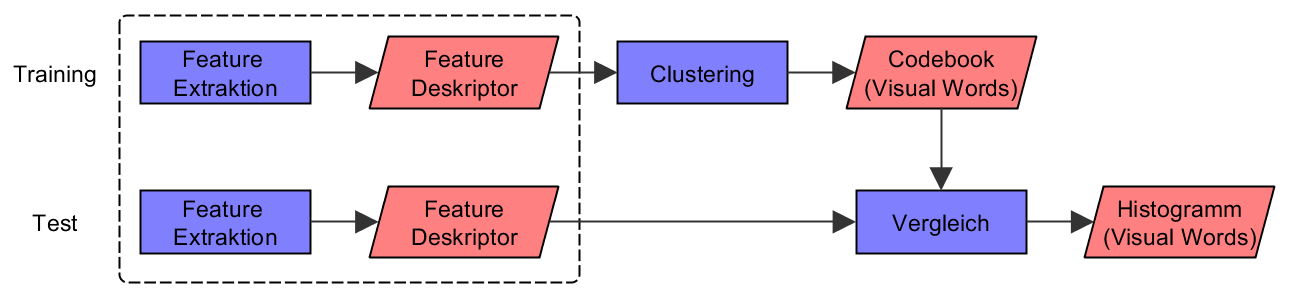
\includegraphics[scale=0.45]{images/bovw.png}
	\caption{Training und Test, bzw. Anwendung, des Bag of Visual Word Modells. \todo{ref}}
	\label{img:bovw}
\end{figure}

\todo{Quelle}

\subsection{Lloyds Algorithmus}

Im Grundlagenkapitel wurde bereits Lloyds Algorithmus eingeführt, hier soll zunächst näher auf die sequentielle Ausführung eingegangen werden, um anschließend eine mögliche Parallelisierung zu diskutieren. Im nachfolgenden Codelisting ist der Ablauf des Algorithmus in Pseudocode beschrieben. Als Parameter werden die Punkte $P$ und die Anzahl der zu bildenden Cluster $k$ erwartet. In Zeile 2 findet die Auswahl der initialen Schwerpunkte der Cluster statt. Die Zuordnung von Punkten zu Clustern erfolgt in Zeile 7: $argminD$ wählt den Cluster aus, dessen Varianz am wenigsten bei Aufnahme des Punktes $p_{i}$ steigt. Abschließend wird die Aktualisierung der Schwerpunkte aller Cluster in Zeile 9 durchgeführt.

\lstset{language=C}
\begin{lstlisting}[mathescape=true]
kmeans_lloyd ($P, C, k$)
	initialisierung
	until convergence
		$C_{j} = 0, j = 1, ..., k$
		for each $p_{i} \in P$
			for each $c_{j} \in C$
				$c_{j} = argminD(c_{j}, p_{i})$		
		for each $c_{j} \in  C$
			$c_{j} = \frac{1}{|c_{j}|} \sum_{n_{i} \in c_{j}} n_{i}$
\end{lstlisting}

Die Initialisierungsphase muss für die Parallelisierung nicht beachtet werden: Sie nimmt nur wenig Zeit in Anspruch und wird einmalig zu Beginn ausgeführt. Die anderen beiden Schritte des Algorithmus bergen mehr Potential: In Zeile 5 bis 7 wird die Varianz jedes Cluster-Vektor Paares berechnet. Da die Berechnung der Varianz eines Paares unabhängig von der eines anderen ist, kann die Berechnung aller Varianzen parallel erfolgen. Nachdem für einen Durchgang die Veränderung der Mitgliedschaft von Vektoren zu Clustern berechnet wurde, müssen die Cluster-Schwerpunkte aktualisiert werden. Auch die Berechnung der neuen Schwerpunkte der Cluster kann unabhängig voneinander erfolgen: Die Vektoren aus denen der Mittelwert berechnet wird, sind genau einem Cluster zugeordnet.

% http://www.know-center.tugraz.at/download\_extern/papers/latex8.pdf

\subsection{Histogramme}

Ein sequentielles Histogramm kann als Programm in einer Schleife über die Daten ausgedrückt werden: Für jedes Element wird der Index der Klasse des Histogramms berechnet und um eins inkrementiert. Zur Normalisierung des Histogramms ist es anschließend notwendig, jede Klasse des Histogramms durch die Gesamtanzahl der Werte zu dividieren. Da es sich bei der Anzahl der Klassen jedoch um eine kleine Zahl, im Vergleich zur Anzahl der Elemente in den Daten, handelt, ist dieser Aufwand vernachlässigbar.
Um das Histogramm der Visual Words eines Bildes zu erzeugen, muss für jedes extrahierte Feature das nächste Visual Word bestimmt werden. Dies entspricht im nachfolgenden Pseudocode der doppelten Schleife über die Features $F$ und Cluster $C$ in Zeile 2 und 3. Der Index des nächsten Clusters wird dann in Zeile 4 durch $argmin D$ berechnet und in der nächsten Zeile wird das Histogramm $H$ an der entsprechenden Stelle inkrementiert.

\begin{lstlisting}[mathescape=true]
histogram ($P, C, H$)
	for each $p_{i} \in P$
		for each $c_{j} \in C$
			$k = arminD(c_{j}, p_{i})$ 
		$H_{k} = H_{k} + 1$		
	for $1 .. |H|$
		$H_{i} = H_{i} / |H|$
\end{lstlisting}

\section{Feature Deskriptoren}
\label{extraction}

Für die weitere Verarbeitung der Features ist es erstrebenswert, dass ihre Darstellung möglichst kompakt ist. Deskriptoren werden als Vektoren von Zahlen kodiert, die abhängig vom Verfahren Informationen über einen Pixel und seine Nachbarschaft oder auch ein ganzes Bild enthalten. Je größer die Anzahl der Einträge eines Vektors, desto größer wird der Speicherbedarf und Rechenaufwand.
Die erste Stufe des vorgestellten Modells, sieht daher die Komprimierung der Feature-Vektoren durch einen Autoencoder vor. Auf diese Weise kann ein initial recht umfangreicher Feature-Vektor aufgebaut werden: Jede Stufe des Autoencoders lernt dann eine kompaktere Darstellung des Feature-Vektors bis zu einer gewünschten Untergrenze.\newline
Da für die vorliegenden Bilddaten der HsH keine speziellen Annahmen getroffen werden können, ist nicht bekannt was für eine Art von Deskriptor gute Ergebnisse liefern kann. In der Literatur findet sich eine große Anzahl an Verfahren zur Detektion und Extraktion von Features für etliche Zwecke. Um einen Überblick zu geben, sollen einige Vertreter angeführt, um den Leser einzuführen.
\newline 
Die Local Binary Patterns (LBP) haben sich im Bereich der Gesichtserkennung erfolgreich etabliert. Eine Region um einen \textit{keypoint} wird hier als ein acht stelliger Bitstring kodiert. Das Verfahren kodiert jeden Pixel einer $3 \times 3$ großen Nachbschaft, außer den Pixel im Fokus, als 0 oder 1, abhängig ob die Intensität größer oder kleiner einem Schwellwert ist.\newline 
Torralba und Olivia \cite{mts2001} haben mit dem  \textit{Spatial Envelope} ein Verfahren entwickelt um die z.B. die Natürlichkeit oder Offenheit einen Szene zu beurteilen. Eine hohe Natürlichkeit weist zum Beispiel auf das Bild einer Landschaft hin: Hier kommen in der Regel kaum gerade vertikale und horizontale Linien vor, im Gegensatz zu Bildern, die von Menschen angefertigt wurden. In dieser Arbeit soll im weiteren eine Basis für das Gruppieren von Bildern durch Features bilden, in dem ein Anwendungsfall umgesetzt wird.
\todo{SIFT, großer Deskriptor}

\begin{itemize}
	\item SIFT toll für Objekterkennung
	\item Coole keypoints aber deskriptor schon zu kompakt für AE
	\item SIFT kps nehmen und daraus eigenen Deskriptor aufbauen
	\item Dann gehts weiter im Konzept mit zusammenflanschen
\end{itemize}